\chapter{Lecture 1: Topics in String Theory}

\lectureoverview{A challenge to reductionism is sharpened through bosonization in \(1+1\) dimensions, electric--magnetic duality, D-branes, strong-coupling transitions, emergent geometry, and the combinatorial landscape of string vacua. The same physical system may admit radically different elementary descriptions; which description looks simple depends on the coupling and the geometry.}

\section{Reductionism, Complexity, and the Question of Simplicity}

Susskind opens with a deliberately familiar philosophical slogan: big things are made of little things, and little things are made of littler things. He then adds the more ambitious version of the same idea, the one that really matters for fundamental physics: as one descends through deeper layers, the objects should become not only smaller but also simpler. His metaphor is that houses are made of bricks, and nobody mistakes a house for a brick. The brick is smaller, but it is also simpler.

The first move of the lecture is to confront that expectation with the actual state of particle physics. If reductionism were delivering increasing simplicity in that strong sense, one might expect present-day elementary particle physics to be close to economical. Instead, Susskind emphasizes that even before quantum gravity enters, the bookkeeping already looks messy. In the lecture these are rough counts, but the roughness is part of the point:
\begin{equation}
N_{\mathrm{species}} \sim 75,
\qquad
N_{\mathrm{independent}} \sim 10\text{--}20,
\qquad
N_{\mathrm{parameters}} \sim 20.
\end{equation}
Even this is not the end of the story. The Standard Model does not contain gravity, does not explain dark matter, does not supply the extra structure needed for inflation, and carries a severe fine-tuning problem. Adding the usual repair mechanisms only increases the count. Supersymmetry is the lecture's example. At the time of the lecture, many physicists hoped that the Large Hadron Collider would expose superpartners; Susskind stresses that the corresponding extension would introduce more than a hundred additional parameters rather than immediately simplifying the bookkeeping. His schematic message is
\begin{equation}
N_{\mathrm{parameters}}^{\mathrm{extended}} \sim 200.
\end{equation}
These numbers are deliberately rough and historical. They serve the argument that a deeper description need not look simpler at the level of its particle inventory and measured constants.

This quantitative complaint is not yet Susskind's main thesis. It is the prelude. The deeper claim, and the one that drives the rest of the lecture, is that modern quantum field theory and string theory do not obviously support a unique, coupling-independent distinction between the bricks and the houses. The next examples are chosen to show that the very meaning of ``elementary'' may depend on which variables are efficient.

\section{Bosonization: A First Breakdown of Fixed Fundamentality}

Susskind's first theoretical example comes from \(1+1\)-dimensional quantum field theory: one dimension of space, one of time. He announces at once that he is not going to derive the equivalence in detail; the point is not the formal proof but the conceptual lesson.

One starts with a field theory of fermions. The fermion field is denoted by \(\psi\). Two nearby fermions can form a bosonic composite, and the corresponding bosonic field is denoted by \(\phi\). At first sight the hierarchy seems straightforward: \(\psi\) is basic, while \(\phi\) is a composite or effective variable. In the lecture the boson is introduced exactly this way, as a field that creates bound pairs of fermions.

What was discovered, however, is that the same theory can be rewritten from the opposite starting point. One may begin with the bosonic field \(\phi\), and then the fermion no longer appears as a point-like constituent. Instead it appears as a kink of the bosonic field, an extended configuration in which \(\phi\) interpolates smoothly between two asymptotic values. The minimum mathematical content of the lecture is this asymptotic structure:
\begin{equation}
\phi(x\to -\infty)=\phi_-,
\qquad
\phi(x\to +\infty)=\phi_+.
\end{equation}
A convenient schematic representative is
\begin{equation}
\phi(x)\approx \frac{\phi_++\phi_-}{2}
+
\frac{\phi_+-\phi_-}{2}\tanh\!\left(\frac{x}{\ell}\right),
\end{equation}
where \(\ell\) is the width of the transition region.

\editorialnote{The hyperbolic-tangent profile is a standard smooth representative of the kink drawn in the lecture, not a formula derived there. The precise bosonization dictionary depends on the model; the conceptual point is the exchange between a fermionic excitation and a topological soliton of a bosonic field.}

The belt analogy in the lecture is precise enough to be worth keeping. A flat belt with no twist is a configuration with no kink. If one rotates one end by \(2\pi\), the belt returns to the same local orientation far away, but in between it must pass through an extended twisted region. That twisted region is the kink. In the bosonic description, the fermion is represented by precisely such an extended object.

The point becomes sharper once a coupling is introduced. Susskind calls it \(G\) in this example. The statement is not that the two descriptions are vaguely related, but that the efficiency of the two descriptions depends on the parameter regime:
\begin{align}
G \ll 1
&\Rightarrow
\ell \text{ small, the kink is tight, and the }\psi\text{-description is efficient},\\
G \gg 1
&\Rightarrow
\ell \text{ large, the kink spreads out, and the }\phi\text{-description is efficient}.
\end{align}
For small \(G\), the kink is tight and the fermion looks like the simple object. As \(G\) increases, the kink broadens and the fermion becomes less point-like. The bosonic variables then become the more economical ones.

\paragraph{Schematic update rule.}
\begin{enumerate}
\item Begin with a fermionic theory described by \(\psi\).
\item Identify bosonic composites described by \(\phi\).
\item Rewrite the same theory entirely in terms of \(\phi\).
\item In the bosonic description, the fermion reappears as a kink of width \(\ell\).
\item For \(G\ll 1\), \(\ell\) is small and the fermionic description is simplest.
\item For larger \(G\), \(\ell\) grows and the bosonic description becomes simplest.
\end{enumerate}

This is the first explicit counterexample to the fixed ``houses and bricks'' picture. The lecture's punchline is not merely that composite objects exist, but that what counts as the elementary variable can change with the coupling.

\section{Electric Charge, Magnetic Monopoles, and Weak versus Strong Coupling}

Susskind next asks whether an analogous story appears in more familiar particle physics. The example is electric charge versus magnetic monopole. An ordinary charged particle, such as the electron, is an electric monopole in this language: a localized source of electric field. The magnetic monopole is introduced by the bar-magnet analogy. If one could somehow isolate the end of a bar magnet without the invisible connecting bar, the field lines would look exactly like those of an electric charge, but magnetic rather than electric.

The relevant control parameter is the fine-structure constant \(\alpha\). In the lecture Susskind treats it heuristically as the square of the electric charge:
\begin{equation}
\alpha \sim e^2.
\end{equation}
He also gives a rough operational interpretation: it measures how readily an electron radiates, and he summarizes that strength by saying that an accelerated electron radiates on the order of ``\(1/100\)'' photons in the relevant sense. In the lecture's own rough numerical language,
\begin{equation}
\alpha \approx 10^{-2}.
\end{equation}
This is not intended as a precision convention; it is a pedagogical way of encoding that electric charge is weak.

\editorialnote{The weak--strong relation has a precise ancestor in Dirac quantization. In one common convention, electric and magnetic charges obey \(e g_m=2\pi n\). Thus a weak electric coupling corresponds to a strong magnetic one, although exact numerical factors and protected mass relations depend on the theory.}

When \(\alpha\ll 1\), the electron is the simple object. Its electric field is weak, its vacuum polarization cloud is dilute, and it looks almost point-like. The magnetic monopole is then the opposite: its field is enormous, its surroundings are violently distorted, and it is broad, complicated, and heavy. Susskind summarizes the situation in precisely this weak--strong style:
\begin{align}
\alpha \ll 1
&\Rightarrow
\text{electron simple, monopole heavy and extended},\\
\alpha \gg 1
&\Rightarrow
\text{monopole simple, electron heavy and structured}.
\end{align}
The lecture does not derive a monopole mass formula. It does not need one. Its point is that as one increases \(\alpha\), the electron's field grows stronger, the electron acquires more structure, and the monopole shrinks and lightens. If \(\alpha\) were pushed far past unity, the convenient description would exchange: the monopole would be the simple object and the electron the complicated one.

That is the field-theory version of the earlier lesson from bosonization. The distinction between basic and composite is not absolute. It depends on the coupling.

\begin{classroomqa}
\audiencequestion{If reductionism is not a reliable guide, why do physicists rely on calculus, which seems to divide a system into arbitrarily small pieces? \lecturetimestamp{00:21:21}}
\lecturerresponse{Calculus asserts smooth variation; it does not identify the fundamental objects of a theory. Quantum fields fluctuate on every distance scale, producing an endless hierarchy rather than a final smooth layer at which one can decide once and for all what is elementary.}
\end{classroomqa}

The exchange continues with the suggestion that the hierarchy resembles a fractal. Susskind accepts the analogy, then sharpens it: quantum fields fluctuate on every scale and are therefore never smooth in the classical sense. This excessive variation is part of what makes quantum field theory mathematically difficult; ordinary calculus must be used with renormalized quantities rather than with a naively smooth microscopic field.

\section{Strings, D-Branes, and the Return of Weak--Strong Duality}

The next transition in the lecture is deliberately naive. If string theory is supposed to be the theory of the fundamental building blocks, then surely the answer must be simple: the building blocks are strings. Susskind states that expectation openly, and then spends the next part of the lecture dismantling it.

\subsection{Why strings are not the whole story}

The first complication is the unavoidable presence of D-branes. A D\(p\)-brane is a \(p\)-dimensional object on which strings can end. The letter \(D\) comes from Dirichlet boundary conditions, but the name is far less important than the role: these objects are part of the theory and cannot be discarded. They are not optional ornaments.

The simplest examples are:
\begin{itemize}
\item a D0-brane, which is point-like,
\item a D1-brane, or D-string, which is string-like,
\item an F-string, the ordinary fundamental string.
\end{itemize}
A D0-brane is a heavy point-like site on which any number of F-strings can end. A D1-brane is a heavy cable-like object, much thicker and more massive per unit length than an F-string, but likewise a place where F-strings can end. At weak coupling the lecture does not present these objects as equally elementary alternatives. The D-branes are introduced as heavy, structured, composite-looking objects that the theory nevertheless forces upon us.

\editorialnote{The odd-brane theory used in this part of the lecture is Type IIB string theory. Its stable D-branes have odd spatial dimension, including D1- and D3-branes. Susskind postpones these names because the duality pattern, not the taxonomy, is the immediate subject.}

\paragraph{Notation.}
Susskind uses \(G\) and \(g\) somewhat loosely in different parts of the lecture. Here \(G\) is reserved for the bosonization example, while \(g\) denotes the string coupling.

The string coupling \(g\) is defined operationally, not axiomatically. It is the parameter that measures the probability that a fluctuating string splits and forms daughter strings. This is why Susskind compares it directly to the role of \(\alpha\) in QED. The lecture also pauses to identify tension with energy per unit length:
\begin{equation}
T=\frac{E}{L}=\frac{M}{L}.
\end{equation}

For an F-string and a D-string, the standard tension formulas make the weak--strong comparison explicit:
\begin{equation}
T_{\mathrm{F1}}=\frac{1}{2\pi\alpha'},
\qquad
T_{\mathrm{D1}}=\frac{1}{2\pi\alpha' g_s},
\qquad
\frac{T_{\mathrm{D1}}}{T_{\mathrm{F1}}}=\frac{1}{g_s}.
\end{equation}
\editorialnote{These tension formulas supply the conventional normalization behind the lecture's qualitative cable-and-thread comparison. They are an editorial addition; the lecture uses only the scaling with coupling.}

\subsection{F-strings and D-strings}

The weak--strong story then repeats itself in string language. At small coupling the F-string is light, thin, and close to the original intuitive image of the fundamental object. The D-string is thick, heavy, and full of F-string structure. As the coupling grows, the F-string splits more readily; the cloud of daughter strings proliferates around it, and it becomes heavier and more complicated. At the same time the D-string has increasing difficulty emitting the now-heavy F-strings, so its surrounding structure thins out and it becomes lighter and more line-like. The lecture's weak--strong map is therefore
\begin{align}
g \ll 1
&\Rightarrow
\text{F-string light and thin,\quad D-string heavy and structured},\\
g \sim 1
&\Rightarrow
\text{F-string and D-string look comparable},\\
g \gg 1
&\Rightarrow
\text{D-string light and thin,\quad F-string heavy and structured}.
\end{align}
Susskind remarks that around \(g\sim 1\) the two descriptions cease to be sharply distinct. Beyond that point they effectively exchange roles. This is the string-theoretic version of the electron--monopole interchange, and its accepted name is S-duality.

The same exchange can be followed after a string closes into a loop. At weak coupling, a small F-string loop is a light particle-like excitation, while the corresponding D-string loop is heavy and complicated. At strong coupling their roles reverse: the D-string loop becomes the light description, and among the resulting light closed-string excitations is the graviton. The lecture uses this example to insist that even the identity of a familiar particle may depend on which side of the duality is used.

The lecture pushes the point one step further. In the idealized theory the coupling is not merely a number to be dialed by hand; it behaves like a field. Schematically,
\begin{equation}
g = g(x).
\end{equation}
Different regions of space can therefore favor different dual descriptions. In one region F-strings are the light variables; in another region D-strings are. In between, nothing is especially simple. That is why, for Susskind, string theory does not restore the simple reductionist picture. It radicalizes the ambiguity.

\editorialnote{In perturbative string theory the local coupling is set by the dilaton, \(g_s(x)=e^{\Phi(x)}\). Writing \(g=g(x)\) is therefore not merely an analogy, although realistic compactifications generally generate a potential that constrains such variations.}

\begin{classroomqa}
\audiencequestion{If the coupling varied enough that D-strings became lighter than F-strings in another region, would the change affect observable spectra? \lecturetimestamp{00:34:15}}
\lecturerresponse{Yes. That is one reason the exactly symmetric, mathematically controlled model being discussed cannot be identified directly with our world. Its lessons concern what consistent quantum theories can do, not a literal spectrum for nature.}
\end{classroomqa}

\begin{classroomqa}
\audiencequestion{Is there an analogous dual description for a D2-brane? \lecturetimestamp{00:34:39}}
\lecturerresponse{Yes, but it is not another D-string-like exchange. The even-brane case will lead to a membrane interpretation and an additional spatial dimension, which is the next construction.}
\end{classroomqa}

\begin{classroomqa}
\audiencequestion{Does a larger probability for a string to split account for the increased internal complexity? \lecturetimestamp{00:34:53}}
\lecturerresponse{Yes. To make the mechanism concrete, return to QED: an electron emits photons, photons fluctuate into charged pairs, and those charged lines radiate again. Increasing the coupling makes that hierarchy less dilute.}
\end{classroomqa}

\subsection{A question-driven return to quantum electrodynamics}

A student then asks whether the larger splitting probability simply means a more complicated structure ``upstream.'' Susskind answers by returning to quantum electrodynamics and drawing the electron's worldline again. This return matters: it shows that the string story is not an isolated curiosity but another instance of the same weak--strong pattern.

\begin{figure}[htbp]
\centering
\begin{tikzpicture}[scale=1.0]
\draw[->] (-1.2,0) -- (3.7,0) node[right] {space};
\draw[->] (0,-0.2) -- (0,4.3) node[above] {time};

\draw[line width=0.9pt] (0,0.2) -- (0,4.0);
\node[left] at (0,3.55) {\(e^{-}\)};

\draw[line width=0.8pt] (0,1.0) -- (0.18,1.08) -- (0.36,0.92) -- (0.54,1.10) -- (0.72,0.94) -- (0.90,1.12) -- (1.08,0.96) -- (1.26,1.14);
\draw[line width=0.8pt] (0,2.35) -- (-0.18,2.43) -- (-0.36,2.27) -- (-0.54,2.45) -- (-0.72,2.29) -- (-0.90,2.47);

\draw[line width=0.8pt] (1.26,1.14) -- (1.48,1.42);
\draw[line width=0.8pt] (1.26,1.14) -- (1.04,1.42);
\draw[line width=0.8pt] (1.48,1.42) -- (1.58,2.10);
\draw[line width=0.8pt] (1.04,1.42) -- (0.94,2.10);
\draw[line width=0.8pt] (0.94,2.10) -- (1.58,2.10);

\draw[line width=0.7pt] (1.58,1.78) -- (1.72,1.84) -- (1.86,1.72) -- (2.00,1.86);
\draw[line width=0.7pt] (0.94,1.78) -- (0.80,1.84) -- (0.66,1.72) -- (0.52,1.86);

\node at (2.35,1.95) {\(\gamma\)};
\node at (-1.15,2.75) {\(\gamma\)};
\end{tikzpicture}
\caption{Schematic QED hierarchy used in the lecture: a point electron emits photons, photons create pairs, and the daughter charged lines radiate again, producing structure at successively shorter scales.}
\end{figure}

The lecture's point is that even a point electron is accompanied by a hierarchy of processes:
\begin{enumerate}
\item an electron emits and absorbs photons,
\item a photon can create an electron--positron pair,
\item the daughter charged lines can themselves emit photons,
\item the hierarchy continues to smaller scales.
\end{enumerate}
For weak coupling this cloud is dilute, so the electron looks almost point-like in the laboratory. For stronger coupling it proliferates, and the electron becomes a structured object. The string story is then presented as a direct analogue of this.

The same later discussion also motivates Susskind's heuristic energy bookkeeping. He insists that the relevant energy is not merely the sum of free-particle contributions. One must also include interaction energy:
\begin{equation}
E_{\mathrm{tot}} = E_e + E_\gamma + E_{\mathrm{int}}.
\end{equation}
Here \(E_{\mathrm{int}}\) is the crucial term. It is what lets the mass of the dressed electron include the energy associated with its surrounding field and virtual structure. The lecture does not turn this into a formal renormalized self-energy derivation. The point is heuristic but essential: the object's mass already includes the interaction energy required to support the complicated cloud around it.

\begin{classroomqa}
\audiencequestion{Where does the energy for the virtual photons and electron--positron pairs come from if an electron does not contain enough free energy to create a real pair? \lecturetimestamp{00:37:01}}
\lecturerresponse{One never starts with a bare electron and later attaches its Coulomb field. The observed electron is a dressed state, and its mass already includes field and interaction energy. In QED the total energy is not the free electron energy plus the free photon energy alone; the interaction term is indispensable. Calling the intermediate pairs virtual is useful, but the energy bookkeeping belongs to the complete interacting state.}
\end{classroomqa}

\begin{classroomqa}
\audiencequestion{When a high-energy probe reveals this structure, has the probe created it rather than discovered something already present? \lecturetimestamp{00:38:59}}
\lecturerresponse{That interpretive distinction can be debated. Operationally, sufficiently energetic scattering has a calculable, nontrivial final state. At weak coupling most events still look simple, while roughly an \(\alpha\)-sized fraction reveal additional radiation or pairs.}
\end{classroomqa}

\begin{classroomqa}
\audiencequestion{When the D1-brane is said to be more massive than the F-string, is its tension also larger? \lecturetimestamp{00:39:37}}
\lecturerresponse{Yes. For an extended string, ``mass'' here means energy per unit length, which is precisely the tension.}
\end{classroomqa}

\begin{figure}[htbp]
\centering

\includegraphics[width=0.72\textwidth]{lecture_01_figure_02.png}
\lectureframe{00:38:22.500}

\vspace{1em}

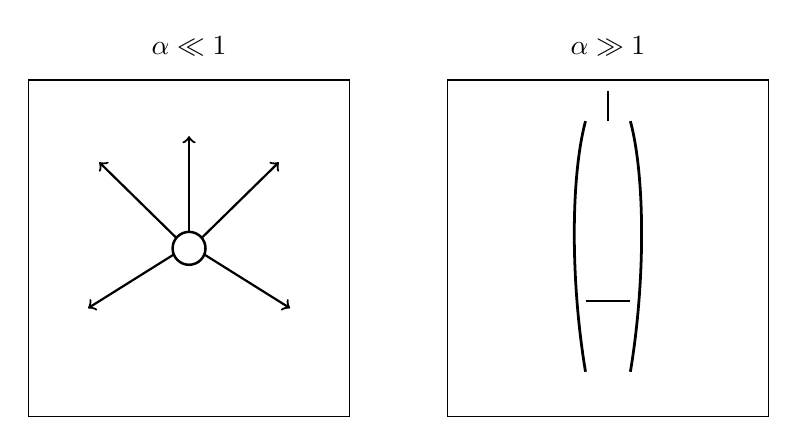
\begin{tikzpicture}[scale=0.95]
\draw (-5.3,-2.4) rectangle (-1.0,2.1);
\draw (0.3,-2.4) rectangle (4.6,2.1);

\node at (-3.15,2.55) {$\alpha \ll 1$};
\node at (2.45,2.55) {$\alpha \gg 1$};

\draw[line width=0.9pt] (-3.15,-0.15) circle (0.22);
\draw[->,line width=0.8pt] (-3.15,0.07) -- (-3.15,1.35);
\draw[->,line width=0.8pt] (-2.98,-0.01) -- (-1.95,1.00);
\draw[->,line width=0.8pt] (-3.32,-0.01) -- (-4.35,1.00);
\draw[->,line width=0.8pt] (-2.95,-0.23) -- (-1.80,-0.95);
\draw[->,line width=0.8pt] (-3.35,-0.23) -- (-4.50,-0.95);

\draw[line width=1.0pt] (2.15,-1.8) .. controls (1.95,-0.6) and (1.95,0.8) .. (2.15,1.55);
\draw[line width=1.0pt] (2.75,-1.8) .. controls (2.95,-0.6) and (2.95,0.8) .. (2.75,1.55);
\draw[line width=0.8pt] (2.15,-0.85) -- (2.75,-0.85);
\draw[line width=0.8pt] (2.45,1.55) -- (2.45,1.95);
\end{tikzpicture}
\caption{The weak--strong QED comparison during the interaction-energy discussion. The diagram isolates the two regimes visible around Susskind: a dilute weak-coupling cloud and a proliferating strong-coupling one.}
\end{figure}

The reason this figure belongs here, even though the weak--strong comparison was introduced earlier, is that in the lecture Susskind redraws the contrast at this later question-driven moment while discussing interaction energy and proliferating structure.

\section{Even-Brane Theories and the Emergent Extra Dimension}

Up to this point the lecture has been telling a strong story about exchange: fermion versus boson, electron versus monopole, F-string versus D-string. The next step is more surprising. Susskind switches to a different version of string theory, one with even-dimensional D-branes rather than odd-dimensional ones. The distinction matters because in this theory there is no D-string to exchange with the F-string. One has D0-branes, D2-branes, D4-branes, and so on.

The strong-coupling limit therefore cannot simply be a relabeling of one string as another. According to the lecture, something stranger happens: an extra spatial dimension becomes manifest. Susskind deliberately states this in the most dramatic form first --- ``a new dimension materializes'' --- and then immediately translates it into the more careful statement: a very small compact direction expands until it can no longer be ignored.

The bookkeeping is part of the point, so he pauses over it:
\begin{equation}
\begin{aligned}
10\text{-dimensional string theory} &= 9\text{ space}+1\text{ time},\\
11\text{-dimensional theory} &= 10\text{ space}+1\text{ time}.
\end{aligned}
\end{equation}
The lecture's claim is that the strong-coupling limit of the even-brane theory is effectively eleven-dimensional.

\editorialnote{The even-brane theory is Type IIA string theory, and its strong-coupling completion is M-theory. In standard units the emergent-circle radius and eleven-dimensional Planck length scale as \(R_{11}=g_s\ell_s\) and \(\ell_{11}=g_s^{1/3}\ell_s\). These names and formulas make explicit the modern dictionary behind the lecture's geometric account.}

\subsection{The peanut-butter sandwich}

To picture the compact direction, Susskind uses the ``peanut-butter sandwich'' model: two infinitely thin pieces of bread, with real space between them. The special rule is that going out one side returns one to the other. In a conventional notation that the lecture describes pictorially rather than formally, one may write
\begin{equation}
y \sim y + 2\pi R.
\end{equation}
If \(R\) is very small, observers living in the sandwich effectively describe their world as lower-dimensional. The key strong-coupling update is then
\begin{equation}
g\uparrow
\qquad \Longrightarrow \qquad
R_{\mathrm{compact}}\uparrow.
\end{equation}
That is what Susskind means when he says that a new dimension of space appears: not that space is created from nothing, but that a previously tiny compact direction expands and becomes visible in the effective theory.

\begin{figure}[htbp]
\centering
\resizebox{\linewidth}{!}{%
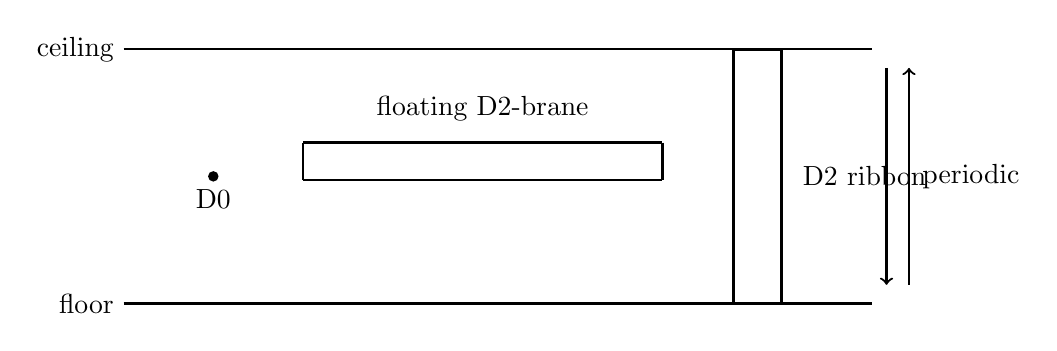
\begin{tikzpicture}[scale=0.95]
\draw[line width=0.9pt] (-5,1.7) -- (5,1.7);
\draw[line width=0.9pt] (-5,-1.7) -- (5,-1.7);

\node[left] at (-5,1.7) {ceiling};
\node[left] at (-5,-1.7) {floor};

\draw[->,line width=0.8pt] (5.2,1.45) -- (5.2,-1.45);
\draw[->,line width=0.8pt] (5.5,-1.45) -- (5.5,1.45);
\node[right] at (5.55,0) {periodic};

\draw[line width=1.0pt] (-2.6,0.45) -- (2.2,0.45);
\draw[line width=1.0pt] (-2.6,-0.05) -- (2.2,-0.05);
\draw[line width=1.0pt] (-2.6,0.45) -- (-2.6,-0.05);
\draw[line width=1.0pt] (2.2,0.45) -- (2.2,-0.05);
\node at (-0.2,0.9) {floating D2-brane};

\draw[line width=1.0pt] (3.15,-1.7) -- (3.8,-1.7);
\draw[line width=1.0pt] (3.15,1.7) -- (3.8,1.7);
\draw[line width=1.0pt] (3.15,-1.7) -- (3.15,1.7);
\draw[line width=1.0pt] (3.8,-1.7) -- (3.8,1.7);
\node[right] at (3.95,0) {D2 ribbon};

\fill (-3.8,0) circle (0.07);
\node[below] at (-3.8,-0.05) {D0};
\end{tikzpicture}
}%
\caption{The sandwich compactification. The upper and lower boundaries are periodically identified; one D2-brane floats between them like a carpet, while another stretches from floor to ceiling and looks string-like when the compact direction is small.}
\end{figure}

\subsection{What becomes of the D0- and D2-branes?}

The lecture now asks what happens to the D0-branes and the strings. The answer is asymmetric. As \(g\) becomes large, the D0-branes get lighter and lighter; in the higher-dimensional interpretation they join the tower of particles carrying momentum in the newly manifest direction. Thus a heavy, complicated object in the weak-coupling picture becomes an ordinary light excitation in the strong-coupling picture.

The mass relation displays the identification:
\begin{equation}
M_{D0}(n)=\frac{n}{g_s\ell_s}
=\frac{n}{R_{11}}
=M_{\mathrm{KK}}(n).
\end{equation}
\editorialnote{Susskind calls the D0-branes ``the gravitons'' of the eleven-dimensional theory. More precisely, their bound states are the Kaluza--Klein momentum modes of the eleven-dimensional supergravity multiplet, whose massless sector contains the graviton. The distinction preserves the lecture's physical identification while avoiding a literal one-particle overstatement.}

The D2-branes explain the fate of the strings. There are two configurations emphasized in the lecture:
\begin{enumerate}
\item a D2-brane floating between floor and ceiling like a carpet in the peanut butter;
\item a D2-brane stretched from floor to ceiling like a ribbon, extended along the visible direction.
\end{enumerate}
When the sandwich is thin, the ribbon looks effectively one-dimensional. It is the object that low-energy observers call a string. As the compact direction opens up, that same object becomes unmistakably membrane-like. Because it now contains more material in the vertical direction, it becomes heavy and unstring-like.

\paragraph{The logic of the transition.}
\begin{enumerate}
\item Start with a very thin compact direction, so the floor-to-ceiling ribbon behaves effectively like a string.
\item Increase \(g\), and the compact direction expands.
\item The D0-branes become light and are reinterpreted as Kaluza--Klein momentum states in the higher-dimensional theory.
\item The string-like D2 ribbon becomes a visibly extended membrane and grows heavy.
\end{enumerate}
This is the lecture's hinge from duality to emergent geometry. Strong coupling does not merely exchange one object for another; it changes which geometry is the efficient one.

Susskind pauses over how strange this sounds. The web of proposed identifications required difficult mathematical consistency relations, some of which first appeared to physicists as conjectures and were later established by mathematicians. His claim is not that every realistic string vacuum is understood, but that the duality web itself has survived unusually stringent checks.

If the coupling varies from place to place in this idealized setting, the efficient geometry can vary with it. One region may look nearly ten-dimensional, with light strings and heavy D0-branes; another may open into the eleven-dimensional description, with heavy wrapped membranes and light Kaluza--Klein modes. The local change of language is part of the same duality web.

The transcript briefly renders the name of these relations as ``inequalities.'' In context the intended word is \emph{dualities}: relationships between opposite ends of parameter space. The correction matters because the lecture's conclusion is precisely that no unique list of fundamental constituents is known. Strings, branes, particles, and higher-dimensional geometry can transform into one another; either no member of the web is absolutely fundamental, or some deeper organization remains unknown.

\section{D3-Branes, Wrapped Membranes, and a Geometrical Picture of Duality}

After the break Susskind explicitly describes the subject as an ``enormous web'' of interconnected theories and ideas. The next examples are not new isolated effects; they are bridges tying together the previous ones.

\subsection{A D3-brane worldvolume}

The first bridge uses a D3-brane. A D3-brane has three spatial dimensions, and an observer confined to it can easily mistake it for ordinary space. The brane can bend and fluctuate, while strings ending on it can join, split, and scatter. To an observer who sees only directions along the brane, each endpoint looks like a particle and the interactions among endpoints look like an ordinary quantum field theory.

\begin{figure}[htbp]
\centering
\resizebox{\linewidth}{!}{%
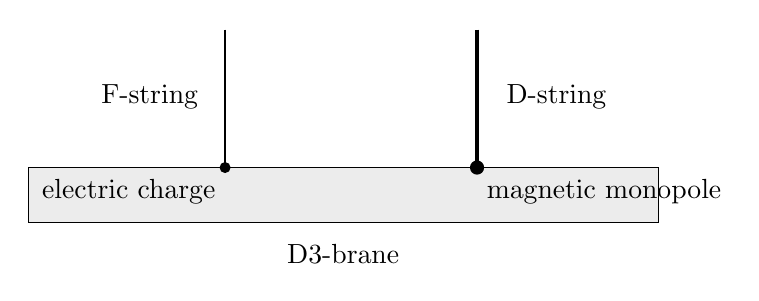
\begin{tikzpicture}[scale=1.0]
\draw[fill=gray!15] (-4,-0.35) rectangle (4,0.35);
\node at (0,-0.75) {D3-brane};

\draw[line width=0.9pt] (-1.5,2.1) -- (-1.5,0.35);
\fill (-1.5,0.35) circle (0.07);
\node[left] at (-1.72,1.25) {F-string};
\node[below left] at (-1.5,0.32) {electric charge};

\draw[line width=1.5pt] (1.7,2.1) -- (1.7,0.35);
\fill (1.7,0.35) circle (0.09);
\node[right] at (1.95,1.25) {D-string};
\node[below right] at (1.7,0.32) {magnetic monopole};
\end{tikzpicture}
}%
\caption{D3-brane worldvolume interpretation. An F-string endpoint appears as an electric charge; a D-string endpoint appears as a magnetic monopole.}
\end{figure}

This is one of the lecture's most satisfying identifications. An F-string ending on the D3-brane appears to the worldvolume observer as an electric charge. A D-string ending on the same brane appears as a magnetic monopole. In other words, the duality between F-strings and D-strings becomes, on the D3-brane worldvolume, the electric--magnetic duality of ordinary field theory. What was earlier an analogy is now an explicit dictionary.

\editorialnote{For a stack of D3-branes, the low-energy worldvolume description is four-dimensional \(\mathcal N=4\) supersymmetric Yang--Mills theory. Its electric--magnetic duality is the field-theory realization of Type IIB S-duality; a single brane gives the Abelian limit used pictorially in the lecture.}

\subsection{Two compact directions and asymmetric wrapping}

Susskind then returns to the higher-dimensional geometry and compactifies not one but two small directions. Since one cannot draw eleven dimensions on a blackboard, he compresses the seven large directions not used in the sketch into one visible horizontal direction, then draws the two compact ones explicitly. He insists on drawing the compactification asymmetrically, because one compact direction must be shorter than the other if the effective strings are to have different tensions.

\begin{figure}[htbp]
\centering

\includegraphics[width=0.78\textwidth]{lecture_01_figure_03.png}
\lectureframe{01:10:25.000}
\caption{The completed board state for the two wrapped membranes. The short and long compact cycles produce the F- and D-string-like ribbons drawn at the right.}
\end{figure}

A membrane may wrap either compact direction and look like a string from the non-compact directions. If \(R_1\) and \(R_2\) are the two circle radii, its effective tensions are
\begin{equation}
T_{(1)}=2\pi R_1 T_{\mathrm{M2}},
\qquad
T_{(2)}=2\pi R_2 T_{\mathrm{M2}},
\qquad
\frac{T_{(1)}}{T_{(2)}}=\frac{R_1}{R_2}.
\end{equation}
Thus unequal circle sizes produce unequal string tensions. With the shorter wrapping identified as the light F-string and the longer one as the heavy D-string, one may write schematically
\begin{equation}
g_s\sim \frac{R_{\mathrm{short}}}{R_{\mathrm{long}}},
\qquad
\frac{T_{\mathrm{D1}}}{T_{\mathrm{F1}}}\sim \frac{1}{g_s}.
\end{equation}

\begin{classroomqa}
\audiencequestion{Can the coupling in this picture be understood as the ratio of the two compact dimensions? \lecturetimestamp{01:10:13}}
\lecturerresponse{Yes. The weak--strong parameter is geometrized as an aspect ratio. Making one direction short produces a small coupling; exchanging the two directions exchanges the light and heavy strings.}
\end{classroomqa}

\editorialnote{The lecture temporarily calls this ratio \(\alpha\), reusing the symbol previously used for the QED fine-structure constant. We write \(g_s\) here to keep the two meanings distinct. In the full M-theory construction the Type IIB coupling is encoded in the complex structure of the compact two-torus; the precise numerator depends on how its cycles are labelled.}

The wrapped-membrane picture can be summarized without the perspective distortion of the blackboard drawing:

\begin{figure}[htbp]
\centering
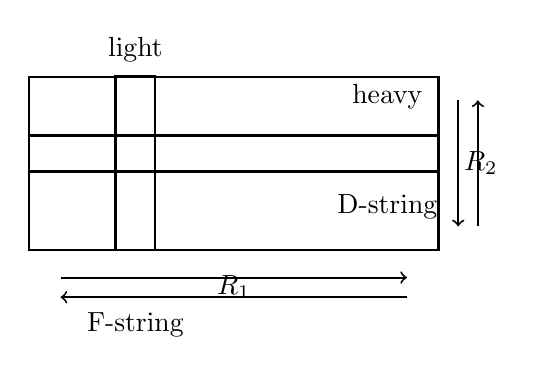
\begin{tikzpicture}[scale=1.0]
\draw[line width=0.9pt] (0,0) rectangle (5.2,2.2);
\node[below] at (2.6,-0.2) {\(R_1\)};
\node[right] at (5.4,1.1) {\(R_2\)};

\draw[->,line width=0.7pt] (5.45,1.9) -- (5.45,0.3);
\draw[->,line width=0.7pt] (5.7,0.3) -- (5.7,1.9);
\draw[->,line width=0.7pt] (0.4,-0.35) -- (4.8,-0.35);
\draw[->,line width=0.7pt] (4.8,-0.6) -- (0.4,-0.6);

\draw[line width=1.0pt] (1.1,0) -- (1.6,0) -- (1.6,2.2) -- (1.1,2.2) -- cycle;
\node at (1.35,2.55) {light};

\draw[line width=1.0pt] (0,1.45) -- (5.2,1.45);
\draw[line width=1.0pt] (0,1.00) -- (5.2,1.00);
\node at (4.55,1.95) {heavy};

\node at (1.35,-0.95) {F-string};
\node at (4.55,0.55) {D-string};
\end{tikzpicture}
\caption{Two wrapped membrane configurations both look string-like from the non-compact directions, but unequal compact scales make one effective string lighter than the other.}
\end{figure}

This is the geometric version of the earlier duality story. Squeezing one direction while stretching the other makes one wrapped object heavier and the other lighter, so the roles of F-string and D-string can interchange.

\begin{classroomqa}
\audiencequestion{If the compact directions are cyclic, are the wrapped objects infinitely wide? \lecturetimestamp{01:10:41}}
\lecturerresponse{No. A compact circle has finite circumference even though one can traverse it repeatedly without reaching an edge. The top and bottom of the cut-open drawing represent the same point, just as the endpoints of an interval can represent one circle point.}
\end{classroomqa}

\begin{figure}[htbp]
\centering

\includegraphics[width=0.78\textwidth]{lecture_01_figure_04.png}
\lectureframe{01:12:25.000}

\vspace{1em}

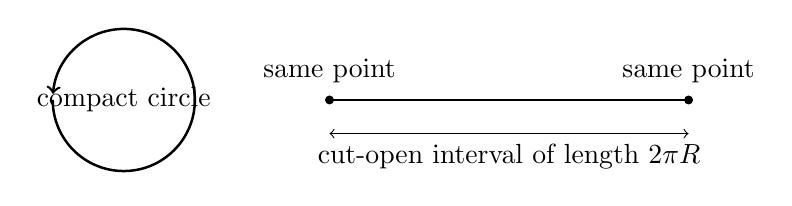
\begin{tikzpicture}[scale=0.95]
\draw[line width=0.9pt,->] (-3.7,0) arc[start angle=180,end angle=535,radius=0.95];
\node at (-2.75,0) {compact circle};
\draw[line width=0.9pt] (0.0,0) -- (4.8,0);
\fill (0.0,0) circle (0.06);
\fill (4.8,0) circle (0.06);
\draw[<->] (0.0,-0.45) -- (4.8,-0.45);
\node at (2.4,-0.75) {cut-open interval of length \(2\pi R\)};
\node[above] at (0.0,0.1) {same point};
\node[above] at (4.8,0.1) {same point};
\end{tikzpicture}
\caption{A compact circle and its cut-open blackboard representation. Crossing one endpoint returns at the other; moving around the circle while also moving in a non-compact direction would instead trace a helix.}
\end{figure}

\begin{classroomqa}
\audiencequestion{Why is the compact path a circle rather than a helix? \lecturetimestamp{01:12:23}}
\lecturerresponse{At each fixed point in the non-compact direction, the compact direction is a circle. A helix appears only if one advances in the non-compact direction while simultaneously winding around the circle. The blackboard interval is simply a circle cut open, with its two endpoints identified.}
\end{classroomqa}

\begin{classroomqa}
\audiencequestion{Does this geometry itself explain how a D-brane can look like a collection of F-strings when probed closely? \lecturetimestamp{01:12:49}}
\lecturerresponse{The connection is present, but it is not transparent in this elementary picture; seeing it requires more geometric machinery. The diagram is meant to organize the duality, not to derive every microscopic constituent description.}
\end{classroomqa}

\begin{classroomqa}
\audiencequestion{Could the long and short compact directions exchange as one moves through space, or as time evolves? \lecturetimestamp{01:13:35}}
\lecturerresponse{Either is possible in the idealized model. Squashing one cycle while expanding the other interchanges which wrapped string is light. This is another reason ``fundamental string'' is only a name: the preferred description can change from region to region or with time.}
\end{classroomqa}

\section{Idealization, Specially Symmetric Points, and the Landscape}

The last movement of the lecture steps back from the elegant duality examples and asks what they do, and do not, tell us about the real world.

First, Susskind warns that the precisely controlled dualities are features of highly idealized supersymmetric theories, in which bosons and fermions occur with exactly matched masses. His analogy is to circular orbits in Newtonian mechanics: one studies them first because they are symmetric and mathematically tractable, not because actual planetary motion is exhausted by perfect circles. In exactly the same way, supersymmetric string theories are easier to analyze because they are more symmetric than nature appears to be.

The idealization is nonetheless informative. A perfect circular orbit is not a realistic planetary system, but it displays features that survive in less symmetric orbits. Likewise, the supersymmetric examples show consistent ways in which quantum mechanics, gravity, and microscopic structure can fit together. Susskind's deliberately sharp formulation is that the tractable string theories are not, literally, the theory of our world; their value is that they reveal phenomena likely to reappear in less symmetric and less tractable settings.

\subsection{A construction kit with many outcomes}

D-branes are only part of the available construction kit. The lecture also names fluxes, orbifolds, and orientifolds. One first chooses a compact geometry, then chooses which branes and fluxes occupy its cycles. Even the simple sandwich changes its lower-dimensional physics when one inserts one floating D2-brane, two of them, or three. Adding or subtracting such ingredients changes the effective particles, interactions, and parameters.

Suppose, in the lecture's schematic count, a six-dimensional compact space has roughly \(500\) cycles and each cycle admits on the order of \(10\) choices of wrapped branes, fluxes, or related structures. Then the number of constructions grows like
\begin{equation}
N_{\mathrm{vacua}} \sim 10^{500}.
\end{equation}
The lecture's counting logic is elementary:
\begin{equation}
10 \times 10 \times \cdots \times 10 = 10^{500}
\end{equation}
with \(500\) factors. The DNA analogy makes the same point in a more familiar register:
\begin{equation}
N_{\mathrm{DNA}}(500)=4^{500}.
\end{equation}
During the DNA comparison, an audience member checks that there are four alternatives along one strand: A, C, G, and T. The correction reinforces rather than changes the argument. A short list of local choices, repeated many times, produces a vast number of global arrangements. The exact exponent is not the point, and Susskind calls \(10^{500}\) an old underestimate; the point is combinatorial proliferation.

This gives the final inversion of the opening reductionist expectation. Complicated particle physics need not arise from complicated microscopic rules. It may arise because our vacuum is one complicated arrangement of many simple ingredients, just as a complicated organism can be encoded by a sequence built from four bases.

\begin{classroomqa}
\audiencequestion{After equivalent descriptions related by duality are identified, would complete information select only one or a few of these possible vacua as descriptions of our world? \lecturetimestamp{01:26:11}}
\lecturerresponse{Presumably it would select a restricted set, but many distinct vacua may look extremely similar at accessible energies. The quoted landscape count is meant to remain large even after dual descriptions are identified, and irrelevant high-energy details may function like ``junk DNA.''}
\end{classroomqa}

\subsection{Symmetric points and generic complexity}

Within the landscape there are specially symmetric points. In the geometric picture an equal-aspect configuration,
\begin{equation}
R_1=R_2,
\end{equation}
makes the two wrapped descriptions equally simple. In the electric--magnetic analogy this is represented schematically by
\begin{equation}
m_{\mathrm{monopole}}=m_e.
\end{equation}

\begin{figure}[htbp]
\centering
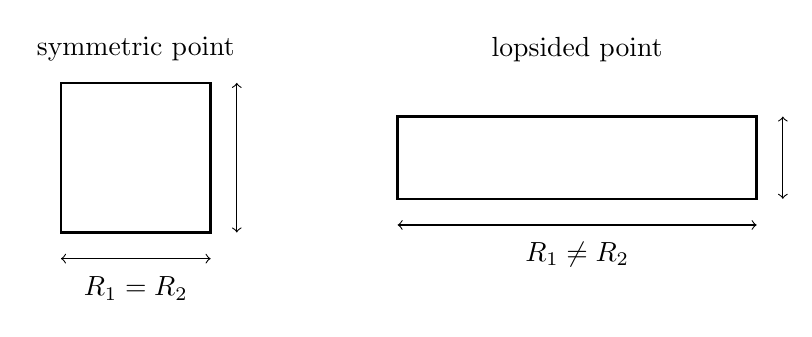
\begin{tikzpicture}[scale=0.95]
\draw[line width=0.9pt] (-4.5,-1.0) rectangle (-2.5,1.0);
\draw[<->] (-4.5,-1.35) -- (-2.5,-1.35);
\draw[<->] (-2.15,-1.0) -- (-2.15,1.0);
\node at (-3.5,1.45) {symmetric point};
\node at (-3.5,-1.75) {$R_1=R_2$};

\draw[line width=0.9pt] (0.0,-0.55) rectangle (4.8,0.55);
\draw[<->] (0.0,-0.9) -- (4.8,-0.9);
\draw[<->] (5.15,-0.55) -- (5.15,0.55);
\node at (2.4,1.45) {lopsided point};
\node at (2.4,-1.3) {$R_1\ne R_2$};
\end{tikzpicture}
\caption{An equal-aspect compactification treats the two wrapped strings symmetrically; a lopsided compactification makes one description much lighter than the other.}
\end{figure}

\begin{classroomqa}
\audiencequestion{Are there vacua in the landscape where the construction becomes much simpler because the F- and D-string descriptions coincide? \lecturetimestamp{01:27:21}}
\lecturerresponse{Yes, there are specially symmetric points. Our world does not appear to sit at one: the familiar electric particle and a magnetic monopole do not have equal masses. Why nature occupies a lopsided point is not known.}
\end{classroomqa}

\editorialnote{The equal electron--monopole mass is a schematic feature of a suitably protected self-dual model, not a prediction of ordinary nonsupersymmetric QED. It expresses the lecture's symmetric-point idea rather than a claim about the observed electron.}

Susskind then recalls an analogy from communication theory. Random codes can be extraordinarily good, while the codes easiest to describe and decode have extra mathematical structure and historically performed less well. Coding theory later found highly effective structured constructions, but the analogy remains: anything compactly named or described occupies a very special, low-complexity corner of the full space of possibilities. Likewise, the string vacua that are easiest to calculate may be atypically simple.

The appropriate questions may therefore change. Instead of demanding the exact compactification in every microscopic detail, one may ask which features are common or generic across a broad ensemble. Susskind presents this as a research problem, not a settled conclusion, and rejects ideological arguments in place of calculation.

\subsection{Cosmological questions}

\begin{classroomqa}
\audiencequestion{Is a compact direction of enormous circumference observationally different from an infinite direction, and do we know that our three large spatial dimensions are infinite? \lecturetimestamp{01:30:03}}
\lecturerresponse{We do not know that they are infinite. A closed three-sphere can expand while remaining compact. Measurements of near-flatness provide only a lower bound on the curvature radius, just as surveying a nearly flat field can bound the Earth's size without proving that its surface is infinite. Only a detected curvature or global identification would determine the finite scale.}
\end{classroomqa}

\begin{classroomqa}
\audiencequestion{If the coupling can vary through space in the idealized model, how could such a variation occur in the real world? \lecturetimestamp{01:32:43}}
\lecturerresponse{Not as the unrestricted smooth variation used in the symmetric example. The realistic possibility to be discussed later is variation by discrete transitions between regions with different effective laws. Whether such jumps occur is a cosmological question.}
\end{classroomqa}

\editorialnote{This response should be read as the lecture's preview of flux vacua and domain transitions, not as a general theorem forbidding every smoothly varying scalar field. Observations strongly constrain variations of dimensionless couplings, while stabilization mechanisms determine whether continuous moduli remain available in a given model.}

The recording does not preserve the final audience question. The surviving response says that the proposed phenomenon can occur for some kinds of black holes but not at the horizon of an ordinary Schwarzschild black hole, whose horizon is locally an ordinary place for a freely falling observer. Because the question cannot be recovered reliably, no more specific claim is attributed to the exchange.

\section{From Bricks to a Web of Descriptions}

The hope that deeper layers of physics must be simpler has proved fragile. In \(1+1\)-dimensional bosonization, the same theory can be organized either around fermions or around bosons, with the fermion reappearing as a kink. In quantum electrodynamics, weak and strong coupling exchange the descriptive roles of electron and magnetic monopole. In string theory, F-strings and D-strings repeat the same pattern, and in the even-brane theory strong coupling goes further still: a compact direction expands, D0-branes become Kaluza--Klein momentum states, and effective strings are reinterpreted as wrapped membranes in a higher-dimensional geometry. Modern quantum field theory and string theory therefore do not furnish a unique once-and-for-all answer to the question ``which are the bricks and which are the houses?'' They furnish a web of descriptions, each efficient in its own regime, together with a huge landscape of possible constructions whose generic output is complexity rather than simplicity.
